\section{Processi di supporto}
\label{processisupporto}

\subsection{Processo di documentazione}
\label{processodocumentazione}
Il processo di documentazione è un processo che consente di registrare le informazioni prodotte dalle attività svolte durante il ciclo di vita del software. Tale processo vuole individuare una strategia per lo sviluppo della documentazione. In particolare, in questa sezione, verranno individuati quali documenti sono necessari come supporto alle attività di sviluppo e verranno presentati gli standard che il gruppo \authorName{} intende adottare per la loro produzione.\\
Il processo di documentazione è composto dalle seguenti attività:
\begin{itemize}
\item \textbf{Pianificazione;}
\item \textbf{Progettazione e sviluppo;}
\item \textbf{Produzione;}
\item \textbf{Manutenzione;}
\end{itemize}

\subsubsection{Pianificazione}
\label{pianificazionedocumenti}
Lo scopo di quest'attività e di identificare quali documenti necessitino di essere prodotti durante il ciclo di vita del software. Per ogni documento, dovrà esserne definito: il titolo, lo scopo, i destinatari e le procedure di gestione.

\paragraph{\underline{Classificazione dei documenti}:} in questo paragrafo verranno definiti i tipi di documenti che si dovranno produrre. Verranno inoltre fornite le norme su come denominarne i file.

\subparagraph{Documenti informali:} si definiscono documenti informali tutti quei documenti che sono ancora in fase di stesura e devono ancora essere approvati dal \projectManager{}.
\\Tali documenti sono ad \emph{esclusivo} uso interno e non potranno essere divulgati a terze parti, prima di essere stati verificati ed approvati.
\\Una volta approvati, i documenti diventeranno formali e pronti per la distribuzione verso l'esterno.
\\Tutti i documenti informali dovranno essere salvati nel repository\glossario{} nell'apposita cartella\footnote{Per maggiori dettagli vedere la sezione \ref{rdocumentazione}.}.
\\Tali documenti devono essere rinominati osservando le seguenti regole: 
\begin{itemize}
\item La prima lettera di ogni parola, che non sia una preposizione, deve essere necessariamente maiuscola;
\item Gli spazi devono essere sostituiti con il carattere \lq\lq{}\_{}\rq\rq{} (underscore);
\item I caratteri accentati devono essere sostituiti con i medesimi caratteri, ma privi di accento.
\end{itemize}
Un esempio di nome è il seguente: \emph{Studio\_di\_Fattibilita.pdf}.

\subparagraph{Documenti formali:} si definiscono documenti formali tutti i documenti che sono stati approvati dal \projectManager{}\footnote{Fatta eccezion per il \emph{Piano di Progetto}, che viene approvato da un qualsiasi altro membro del gruppo.} e sono pronti per essere rilasciati.
\\Quando un documento diventa formale potrà essere visionato da terze parti.
\\Il file pronto per il rilascio dovrà seguire le stesse norme di nomenclatura del file in fase di stesura con l'aggiunta, alla fine del nome, della versione separata dal carattere \lq\lq{}-\rq\rq{} (trattino) e preceduta da una \lq\lq{}v\rq\rq{} (es. \emph{Studio\_di\_Fattibilita-v1.0.0.pdf}).

\paragraph{\underline{Studio di fattibilità}:} lo scopo di tale documento è di riassumere le considerazioni che portano il gruppo \authorName{} all'accettazione o meno di una proposta per lo sviluppo di un progetto. Nel momento in cui si debba decidere tra svariate proposte, è consentita la stesura di un documento riassuntivo contenente le considerazioni di tutte le proposte.\\
L'uso del documento è interno e la lista di distribuzione comprende solo i committenti.

\paragraph{\underline{Norme di progetto}:} lo scopo di tale documento è di raccogliere le norme, le procedure e gli strumenti di sviluppo che il gruppo \authorName{} intende adottare nel momento in cui venga accettata la produzione di un nuovo progetto.\\
L'uso del documento è interno e la lista di distribuzione comprende solo i committenti.

\paragraph{\underline{Piano di progetto}:} lo scopo di tale documento è di specificare la pianificazione dei lavori durante lo svolgimento di un progetto, pianificare le tempistiche di attuazione delle attività, preventivare e mettere a consuntivo le risorse necessarie ed infine definire una politica di gestione dei rischi.\\
L'uso del documento è esterno e la lista di distribuzione comprende i committenti ed i proponenti.

\paragraph{\underline{Piano di Qualifica}:} lo scopo di tale documento è di descrivere le strategie che il team intende adottare, al fine di perseguire gli obiettivi di qualità che si vogliono ottenere all'eventuale progetto in corso. In questo documento, saranno inoltre presenti i resoconti dell'attività di verifica e le pianificazioni dei vari test che si andranno ad implementare.\\
L'uso del documento è esterno e la lista di distribuzione comprende i committenti ed i proponenti.

\paragraph{\underline{Analisi dei requisiti}:} lo scopo di tale documento è di fornire un prospetto dell'analisi che verrà effettuata sulla proposta di sviluppo di un progetto, al fine di individuarne i requisiti. Il documento conterrà la lista dei casi d'uso e dei requisiti individuati, oltre ai diagrammi delle attività riguardanti le interazioni tra utenti e sistema.\\
L'uso del documento è esterno e la lista di distribuzione comprende i committenti ed i proponenti.

\paragraph{\underline{Specifica tecnica}:} lo scopo di tale documento è di definire la progettazione ad alto livello del sistema che il gruppo \authorName{} ha eventualmente deciso di sviluppare. Il documento conterrà la descrizione delle varie componenti necessarie al sistema, individuate dai \textit{Progettisti}, corredate dai relativi design pattern\g{} utilizzati.\\
L'uso del documento è esterno e la lista di distribuzione comprende i committenti ed i proponenti.

\paragraph{\underline{Definizione di prodotto}:} lo scopo di tale documento è di definire la progettazione di dettaglio del sistema che il gruppo \authorName{} ha eventualmente deciso di sviluppare. Il documento avrà un grado di dettaglio tale da permettere ai \textit{Programmatori} di poter codificare le varie unità software.\\
L'uso del documento è esterno e la lista di distribuzione comprende i committenti ed i proponenti.

\paragraph{\underline{Glossario}:} lo scopo di tale documento è di raccogliere i termini particolari presenti nei vari documenti, che necessitano di un approfondimento. In questi sono presenti gli acronimi e i termini tecnici non immediatamente comprensibili ai lettori della documentazione.\\
L'uso del documento è esterno e la lista di distribuzione comprende i committenti ed i proponenti.

\paragraph{\underline{Verbali}:} lo scopo di tali documenti è di raccogliere le informazioni salienti che emergono dalle riunioni esterne ed interne del gruppo. Le decisioni che verranno prese durante le riunioni dovranno essere tracciate.\\
Tutti i verbali esterni saranno redatti dal \projectManager{}, mentre i verbali interni saranno redatti da un qualsiasi membro presente all'incontro.
\\I verbali dovranno essere denominati secondo il seguente criterio:
\begin{center}
	\textbf{Verbale\{numero del verbale\}\_\{tipo di incontro\}\_\{data incontro\}}
\end{center}
dove:
\begin{itemize}
\item \textbf{Numero del verbale:} indica un numero progressivo che identifica il verbale\footnote{Tale numero dovrà partire da uno.};
\item \textbf{Tipo di incontro:} indica il tipo di incontro avvenuto, che potrà essere:
\begin{itemize}
\item \textbf{Interno:} nel caso si tratti di un incontro interno;
\item \textbf{Esterno:} nel caso si tratti di un incontro esterno.
\end{itemize}
\item \textbf{Data incontro:} indica la data in cui è avvenuto l'incontro\footnote{La data dovrà essere formattata come indicato in sezione \ref{fricorrenti}.}.
\end{itemize}
L'uso del documento è interno, quando si riferisce ad una riunione interna, viceversa è ad uso esterno. La lista di distribuzione comprende sempre sia committenti che proponenti.

\paragraph{\underline{Manuale utente}:} lo scopo di tale documento è di fornire all'utente finale la descrizione dettagliata di tutte le funzionalità che il prodotto offrirà.

\paragraph{\underline{Procedure di gestione dei documenti}:} nel seguente paragrafo sono riportate l'elenco di procedure e regole seguite dal gruppo \authorName{} per la gestione dei documenti.

\subparagraph{Creazione di un documento:}
la creazione di un nuovo documento è a discrezione esclusiva del \projectManager. Nel momento in cui sia necessario creare un nuovo documento, egli dovrà seguire la seguente procedura (fig. \ref{proc_creazione}):
\begin{enumerate}
\item Creare una nuova cartella all'interno di Documenti/ e denominarla con lo stesso nome del documento che si vuole creare;
\item Copiare la cartella \textit{doc}\_\textit{to}\_\textit{modify} (contenuta nella cartella \textit{Template/}) ed il suo contenuto, all'interno della cartella creata al punto 1;
\item Creare una cartella \textit{Content} all'interno della cartella creata al punto 1. Questa directory conterrà i file di compilazione corrispondenti alle varie sezioni del documento;
\item Rinominare il file \textit{template.tex} presente nella cartella \textit{doc}\_\textit{to}\_\textit{modify}, utilizzando lo stesso nome del documento che si vuole creare. Successivamente, spostarlo all'interno della cartella creata al punto 1;
\item Compilare i campi dei file template precedentemente copiati, in base al documento che si vuole creare;
\item Creare i vari file di compilazione corrispondenti alle sezione del documento all'interno della cartella \textit{Content}.
\end{enumerate}
\begin{figure}[!h]
\centering
	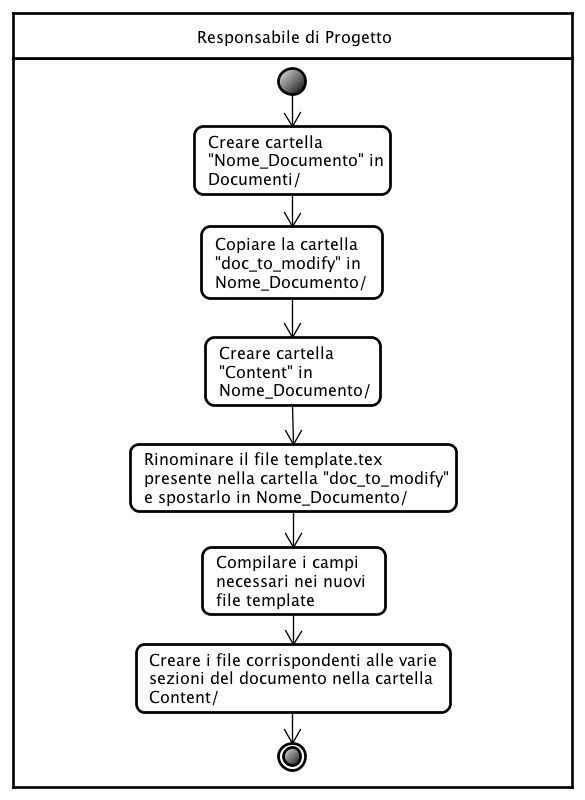
\includegraphics[scale=0.5]{./content/Immagini/Creazione_Doc.png}
	\caption{Procedura di creazione di un documento}
	\label{proc_creazione}
\end{figure}

\subparagraph{Avanzamento di un documento:}
ogni qualvolta un redattore ritiene che la stesura di un documento sia terminata andrà seguita la seguente procedura (fig. \ref{proc_avanzamento}):
\begin{enumerate}
\item Il redattore dovrà contattare il \projectManager{} per informarlo della terminazione della redazione del documento;
\item Il \projectManager{} provvederà ad assegnare la verifica del documento ad uno dei \emph{Verificatori} disponibili che non sia in conflitto d'interessi;
\item Il \emph{Verificatore} provvederà alla verifica del documento;
\item Se sono stati trovati errori, il \emph{Verificatore} provvederà alla creazione di un ticket di correzione.
Successivamente il redattore correggerà gli errori trovati e infine si torna al passo uno;
\item Altrimenti il documento verrà approvato dal \projectManager{}.
\end{enumerate}
\begin{figure}[!h]
\centering
	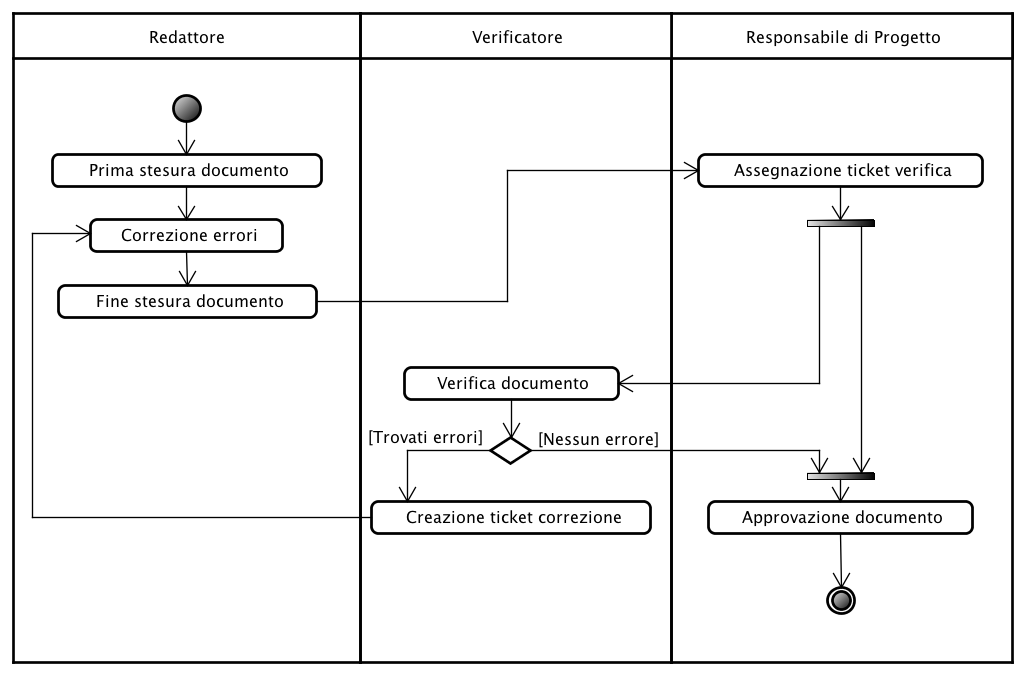
\includegraphics[scale=0.5]{./content/Immagini/Avanzamento_Documento.png}
	\caption{Procedura di avanzamento di un documento}
	\label{proc_avanzamento}
\end{figure}

\paragraph{\underline{Procedure di gestione del Glossario}:} di seguito verranno elencate le procedure specifiche per la gestione del Glossario.

\subparagraph{Inserimento di un termine:}
per l'inserimento di un termine nel \emph{Glossario} si dovrà seguire la seguente procedura (fig \ref{diagramma_add}):
\begin{enumerate}
\item Prima dell'inserimento di un termine andrà contattato il \projectManager{} per proporre l'inserimento del termine;
\item Solo nel caso in cui il \projectManager{} approvi l'inserimento del termine, esso andrà inserito nel \emph{Glossario} nell'ordine lessicografico corretto;
\item Successivamente all'inserimento, si dovrà provvedere a evidenziare ogni occorrenza del termine nei vari documenti.
\end{enumerate}
\begin{figure}[!h]
\centering
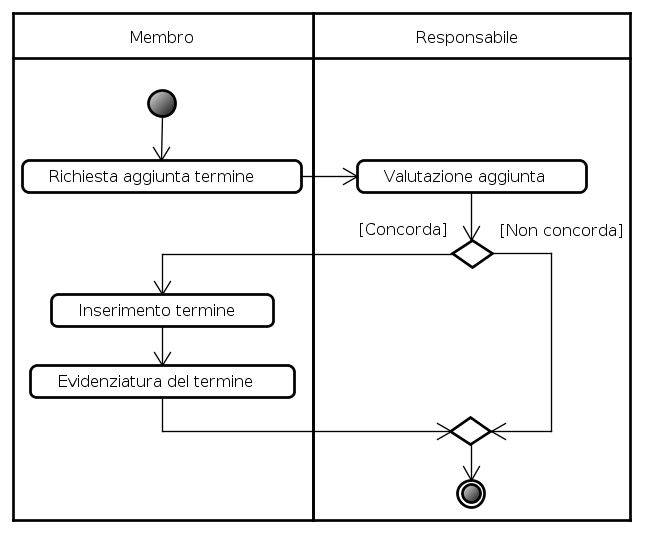
\includegraphics[scale=0.5] {./content/Immagini/Aggiunta_Termine.png}
\caption{Procedimento per l'inserimento di un termine.}
\label{diagramma_add}
\end{figure}

\subparagraph{Eliminazione di un termine:}
ogni membro del gruppo per richiedere l'eliminazione di un termine del \emph{Glossario} dovrà seguire la seguente procedura (fig. \ref{proc_eliminazione}):
\begin{enumerate}
\item Dovrà essere contattato il \projectManager{} per proporre l'eliminazione;
\item Nel caso in cui il \projectManager{} approvi, il termine andrà cancellato dal \emph{Glossario};
\item Successivamente si provvederà a togliere tutte le marcature del termine, all'interno di tutti i documenti.
\end{enumerate}
\pagebreak
\begin{figure}[!h]
\centering
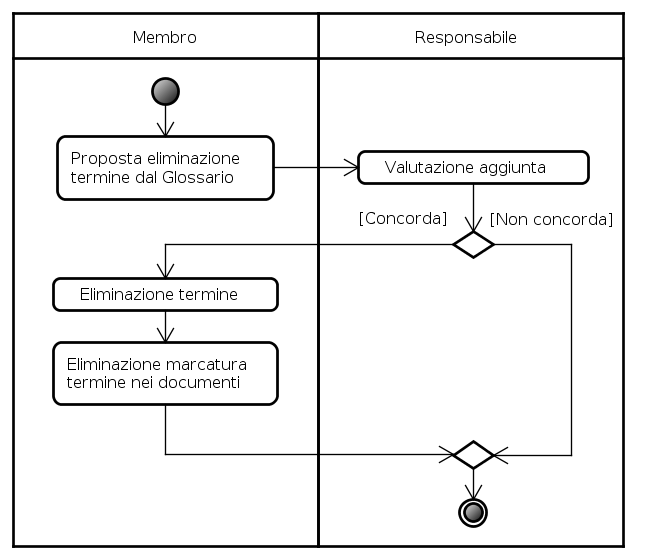
\includegraphics [scale=0.5]{./content/Immagini/Eliminazione_Termine.png}
\caption{Procedimento per l'eliminazione di un termine}
\label{proc_eliminazione}
\end{figure}

\subsubsection{Progettazione e sviluppo}
\label{progettazionesviluppo}
Lo scopo di quest'attività è di definire la struttura del layout dei documenti, le informazioni che devono essere inserite nelle prime pagine, le norme di versionamento, la composizione delle sezioni da inserire e le norme tipografiche a cui si dovranno attenere i redattori.

\paragraph{\underline{Versionamento}:}
ogni documento deve specificare la propria versione, la quale sarà della seguente forma:
\begin{displaymath}
X.Y.Z
\end{displaymath}
dove:
\begin{itemize}
\item\textbf{X:} numero che identifica la versione di rilascio. Ogni incremento causa l'azzeramento dei valori Y e Z. In particolare, questo parametro verrà incrementato ogni qual volta si consegneranno i documenti per una revisione;
\item\textbf{Y:} numero che indica l'avvenuta verifica del documento. Nel momento in cui il verificatore ha controllato il documento, sarà tenuto ad incrementare questo parametro. Ogni incremento inoltre, comporta l'azzeramento del parametro Z;
\item \textbf{Z:} numero che identifica una semplice modifica del documento. Ogni aggiunta o correzione al documento, comporta un incremento del parametro Z.
\end{itemize}

\paragraph{\underline{Template}:}
per facilitare la stesura e la manutenzione dei vari documenti, i file di compilazione sono stati strutturati in maniera tale che la composizione generale sia gestita da template validi per ogni documento. In particolare sono stati creati template per il frontespizio, per il layout, per i comandi utilizzati nei file e per la tabella delle modifiche. Ogni documento avrà una cartella interna denominata \textit{Content}, in cui verranno collocati i file corrispondenti alle varie sezioni che lo compongono.

\paragraph{\underline{Struttura dei documenti}:}
di seguito vengono elencate le norme riguardanti la strutturazione e la suddivisione in sezioni dei vari documenti.

\subparagraph{Prima pagina:}
ogni documento deve avere una prima pagina contenete le seguenti informazioni:
\begin{itemize}
\item Nome del progetto;
\item Logo del gruppo;
\item Nome del gruppo;
\item E-mail esterna del gruppo;
\item Nome del documento;
\item La versione del documento\footnote{Espressa come indicato nel paragrafo \textit{Versionamento} della sezione \ref{progettazionesviluppo}.};
\item Data di redazione del documento;
\item Cognome e nome dei redattori del documento;
\item Cognome e nome dei verificatori del documento;
\item Cognome e nome di chi ha approvato il documento;
\item Tipo d'uso del documento\footnote{Potrà essere interno o esterno.};
\item La lista di distribuzione del documento;
\item Un sommario, contenente una breve descrizione del documento.
\end{itemize}

\subparagraph{Diario delle modifiche:}
nella seconda pagina di ogni documento deve essere presente il diario delle modifiche.
\\Ogni riga del diario delle modifiche deve contenere le seguenti informazioni:
\begin{itemize}
\item Una breve descrizione sulle modifiche effettuate;
\item Il cognome e nome di chi ha effettuato la modifica;
\item Il ruolo dell'autore della modifica;
\item La data in cui è stato modificato il documento\footnote{La data deve essere espressa come riportato nel paragrafo \textit{Formati ricorrenti} in sezione \ref{progettazionesviluppo}.};
\item La versione del documento dopo la modifica.
\end{itemize}

\subparagraph{Indici:}
in ogni documento, tranne che nel \emph{Glossario}, deve essere presente un indice delle sezioni. Nel caso in cui il documento contenga immagini e/o tabelle, devono essere presenti anche i relativi indici.

\subparagraph{Formattazione di una pagina:}
l'intestazione di ogni pagina deve avere le seguenti informazioni:
\begin{itemize}
\item Il logo del gruppo;
\item Nome del gruppo;
\item La sezione corrente all'interno del documento.
\end{itemize}
A piè di pagina deve invece esserci:
\begin{itemize}
\item Nome del documento;
\item La versione corrente del documento;
\item Numero di pagina nel formato \lq\lq{}\textbf{Pagina X di N}\rq\rq{}, dove \lq\lq{}X\rq\rq{} è il numero della pagina corrente e \lq\lq{}N\rq\rq{} è il numero di pagine totali del documento.
\end{itemize}

\paragraph{\underline{Suddivisione sezioni documenti}:} in questo paragrafo verranno definite le principali sezioni che dovranno essere inserite nei documenti e i contenuti che ogni sezione dovrà avere. Per ogni documento saranno descritte sommariamente le sezioni al netto di frontespizio, diario delle modifiche, indice ed introduzione, in quanto sono sezioni comuni a tutti i documenti.

\subparagraph{Studio di fattibilità:} per ogni proposta di progetto dovranno essere presenti le seguenti sezioni:
\begin{itemize}
\item \textbf{Descrizione del capitolato:} contiene una descrizione sommaria del progetto;
\item \textbf{Studio del dominio:} diviso in dominio applicativo e tecnologico, contiene le considerazioni riguardanti il contesto in cui si colloca il prodotto da sviluppare;
\item \textbf{Valutazione complessiva:} diviso in aspetti positivi e negativi, contiene le motivazioni per cui sarebbe fattibile o meno intraprendere lo sviluppo del progetto presentato.
\end{itemize}

\subparagraph{Norme di progetto:} questo documento dovrà essere suddiviso nelle seguenti sezioni:
\begin{itemize}
\item \textbf{Processi primari:} contenente le norme riguardanti i processi primari implementati dal team;
\item \textbf{Processi di supporto:} contenente le norme riguardanti i processi di supporto implementati dal team;
\item \textbf{Processi organizzativi:} contenente le norme riguardanti i processi organizzativi implementati dal team;
\item \textbf{Strumenti:} contenente la lista degli strumenti che il team utilizzerà durante lo sviluppo del progetto. In questa sezione verranno inoltre descritte le principali procedure di interazione che i componenti del gruppo avranno con tali strumenti.
\end{itemize}

\subparagraph{Piano di progetto:} questo documento dovrà essere suddiviso nelle seguenti sezioni:
\begin{itemize}
\item \textbf{Pianificazione:} contenente l'analisi dei rischi del progetto, la pianificazione dello svolgimento delle attività individuate e la suddivisione delle ore necessarie ad ogni ruolo e per ogni attività; 
\item \textbf{Suddivisione del lavoro e proposta economica:} contenente la suddivisione dei ruoli in base alle risorse disponibili ed il prospetto economico delle ore preventivate per i ruoli, in ogni fase;
\item \textbf{Consuntivo corrente:} contenente il bilancio corrente tra preventivo e consuntivo;
\item \textbf{Organigramma:} contenente le informazioni del team.
\end{itemize}

\subparagraph{Piano di qualifica:} questo documento dovrà essere suddiviso nelle seguenti sezioni:
\begin{itemize}
\item \textbf{Visione generale della strategia di verifica:} contiene la definizione degli obiettivi di qualità di processo e prodotto, la pianificazione delle attività di verifica in base alle risorse disponibili e la definizione delle metriche impiegate durante tale attività;
\item \textbf{Gestione amministrativa della revisione:} contiene la strategia di gestione delle procedure che garantiscono la qualità di processo e prodotto;
\item \textbf{Resoconto delle attività di verifica:} appendice contenente gli esiti delle attività di verifica effettuate durante le fasi del progetto;
\item \textbf{Pianificazione dei test:} appendice contenente il tracciamento dei test effettuati sul prodotto software;
\end{itemize}

\subparagraph{Analisi dei requisiti:} questo documento dovrà essere suddiviso nelle seguenti sezioni:
\begin{itemize}
\item \textbf{Descrizione generale:} contiene una descrizione mediamente dettagliata del contesto d'uso del prodotto, delle funzioni che esso dovrà avere e delle caratteristiche generali degli utenti finali;
\item \textbf{Casi d'uso:} contiene l'elenco dei casi d'uso individuati durante l'analisi dei requisiti, corredati dalle relative informazioni;
\item \textbf{Diagrammi delle attività:} contiene una serie di diagrammi di attività che esplicheranno le possibili interazioni che gli utenti potranno avere con il prodotto finito;
\item \textbf{Requisiti:} contiene la lista dei requisiti individuati, corredati da una serie di tabelle che riassumeranno il tracciamento con le fonti e con i test di validazione.
\end{itemize}

\subparagraph{Specifica tecnica:}
\label{parspecificatecnica}
 questo documento dovrà essere suddiviso nelle seguenti sezioni:
\begin{itemize}
\item \textbf{Tecnologie utilizzate:} contiene una panoramica delle tecnologie che verranno utilizzate nell'eventuale sviluppo di un progetto;
\item \textbf{Descrizione architettura:} contiene una panoramica generale dell'architettura che si intende implementare in un eventuale sviluppo di progetto;
\item \textbf{Componenti e classi:} contiene un elenco strutturato che descrive in dettaglio le varie componenti che si intendono implementare nell'architettura del sistema software;
\item \textbf{Design pattern:} contiene la specifica d'uso dei design pattern\g{} che si intendono utilizzare all'interno dell'architettura software;
\item \textbf{Stime di fattibilità e risorse necessarie:} contiene il resoconto delle stime di fattibilità e delle risorse necessarie all'implementazione dell'architettura;
\item \textbf{Tracciamento:} contiene le tabelle di tracciamento tra requisiti e componenti;
\item \textbf{Descrizione dei design pattern:}  appendice contenente una descrizione generale dei design pattern\g{} utilizzati nell'architettura.
\end{itemize}

\subparagraph{Definizione di prodotto:}
\label{pardefinizioneprodotto}
 questo documento dovrà essere suddiviso nelle seguenti sezioni:
\begin{itemize}
\item \textbf{Specifica componenti:} contiene le descrizioni dettagliate delle classi di cui è composto il software.
\end{itemize}

\subparagraph{Glossario:} questo documento dovrà essere suddiviso raggruppando i termini in ordine alfabetico.

\subparagraph{Verbali:} la prima pagina di ogni verbale deve contenere le seguenti informazioni:
\begin{itemize}
\item \textbf{Data}\footnote{Formato espresso come in paragrafo \textit{Formati ricorrenti} della sezione \ref{progettazionesviluppo}};
\item \textbf{Luogo ritrovo:} sintetica descrizione del luogo, correlata da indirizzo e città;
\item \textbf{Ora inizio-fine:} espresso nel seguente formato ora inizio-fine: hh:mm-hh:mm;
\item \textbf{Membri assenti:} i membri assenti alla riunione.
\end{itemize}

\paragraph{\underline{Norme tipografiche}:}
\label{norme tipografiche}
al fine di evitare incoerenza tra le diverse parti dei documenti, si rimanda a questa sottosezione per tutte le informazioni riguardanti l'ortografia, la tipografia e l'assunzione di uno stile uniforme in tutti i documenti.	

\subparagraph{Stile di testo:}
\label{stile}
\begin{itemize}
\item \textbf{Grassetto:} il grassetto si deve utilizzare nei seguenti casi:
\begin{itemize}
\item \textbf{Elenchi puntati:} per evidenziare l'oggetto trattato nel paragrafo;
\item \textbf{Altri casi:} è inoltre possibile utilizzare il grassetto per evidenziare termini particolarmente rilevanti. 
\end{itemize}
\item \textbf{Corsivo:} il corsivo deve essere utilizzato nei seguenti casi:
\begin{itemize}
\item \textbf{Ruoli:} ogni riferimento a un ruolo deve essere scritto in corsivo (esempio: \projectManager);
\item \textbf{Citazioni:} ogni citazione ad una fonte esterna va fatta tramite l'uso del corsivo;
\item \textbf{Documenti:} ogni riferimento a un documento deve essere scritto in corsivo (esempio: \emph{Glossario});
\item\textbf{File e directory:} ogni trascrizione del nome di un file o di una directory, deve essere fatta usando il corsivo; 
\item \textbf{Altri casi:} in altri casi può essere necessario usare il corsivo, come per evidenziare termini particolarmente significativi.
\end{itemize}
\item \textbf{Maiuscolo:} l'uso del maiuscolo è strettamente limitato alla trascrizione di acronimi;
\item \textbf{\LaTeX{}:} ogni riferimento a \LaTeX{} va fatto tramite il comando \verb!\LaTeX!.
\end{itemize}

\subparagraph{Punteggiatura:}
\label{punteggiatura}
\begin{itemize}
\item \textbf{Punteggiatura:} qualsiasi segno di punteggiatura non può seguire un carattere di spazio;
\item \textbf{Punti ellittici:} i punti di sospensione devono essere inseriti esclusivamente tramite il comando \LaTeX{} \verb!\dots!, immediatamente dopo l'ultimo carattere non di spaziatura;
\item \textbf{Parentesi:} il periodo racchiuso tra le parentesi non deve mai iniziare con un carattere di spazio e non deve mai terminare con un carattere di spazio o punteggiatura;
\item \textbf{Lettere maiuscole:} le lettere maiuscole vanno poste dopo il punto, il punto esclamativo, il punto interrogativo e all'inizio di ogni elemento di un elenco puntato. Inoltre viene utilizzata la lettera maiuscola per i ruoli di progetto, i nomi dei documenti, le fasi di progetto, le revisioni di progetto, oltre che dove imposto dalla lingua italiana.
\end{itemize}

\subparagraph{Composizione del testo:}
\label{composizione del testo}
\begin{itemize}
\item \textbf{Elenchi:} la prima parola che segue l'oggetto di indentazione deve avere la prima lettera minuscola. Ogni punto dell'elenco deve terminare con un carattere di punto e virgola, tranne l'ultimo che termina con un punto;
\item \textbf{Note a piè di pagina:} ogni nota a piè di pagina deve iniziare con la prima lettera della prima parola maiuscola non preceduta da caratteri di spazio. Ogni nota a piè di pagina deve terminare con un punto;
\item \textbf{Pedice \lq\lq{}G\rq\rq{}:} il pedice\glossario{} viene utilizzata in corrispondenza di termini tecnici e acronimi presenti nei documenti \emph{Glossario}\footnote{Le occorrenze dei termini presenti nei titoli, nelle note a piè di pagina e negli oggetti degli elenchi non andranno evidenziati.}. 
\end{itemize}

\subparagraph{Formati ricorrenti:}
\label{fricorrenti}
\begin{itemize}
\item \textbf{Nomi propri:} l'utilizzo dei nomi propri deve seguire la forma \lq\lq{}Cognome Nome\rq\rq{};
\item \textbf{Path:} per inserire indirizzi web o indirizzi mail, deve essere utilizzato \emph{esclusivamente} il comando \LaTeX{} \verb!\url!;
\item \textbf{Date:} ogni data deve essere espressa seguendo lo standard ISO 8601\footnote{\url{http://it.wikipedia.org/wiki/ISO_8601}}: 
\begin{displaymath}
	AAAA-MM-GG
\end{displaymath}
dove:
\begin{itemize}
\item \textbf{AAAA:} rappresenta il formato dell'anno scritto con tutte e quattro le cifre;
\item \textbf{MM:} rappresenta il mese scritto con esattamente due cifre\footnote{Nel caso lo si possa scrivere utilizzando solo una cifra, si impone di anteporre uno zero al numero.};
\item \textbf{GG:} rappresenta il giorno scritto con esattamente due cifre.\footnote{Vedi la nota precedente.}
\end{itemize}
\item \textbf{Riferimenti ai documenti:} ci si riferirà ai vari documenti scrivendoli in corsivo e mettendo una lettera maiuscola per ogni parola che non sia un articolo (ad esempio \emph{Norme di Progetto}). 
\\Nel caso ci sia la necessità di riferirsi ad una versione specifica del documento, essa andrà indicata (esempio: \NdP{});
\item \textbf{Nomi propri:} i nomi propri di persona devono essere scritti nel formato \lq\lq{}Cognome Nome\rq\rq{};
\item \textbf{Nome del gruppo:} ci si riferirà al gruppo Seven Monkeys con la dicitura \lq\lq{}\authorName{}\rq\rq{}, con il nome del gruppo in corsivo. Per la corretta scrittura è stato creato un comando \LaTeX{} apposito \verb!\authorName!;
\item \textbf{Nome del proponente:} ci si riferirà al proponente con \lq\lq{}Department of Information Engineering\rq\rq{}. Per la corretta scrittura è stato creato il comando \verb!\proposerName!;
\item \textbf{Nome del progetto:} ci si riferirà al progetto solo con \lq\lq{}\project\rq\rq{}. Per la corretta scrittura è stato creato il comando \LaTeX{} apposito \verb!\project!;
\item \textbf{Sigle:} le sigle andranno usate \emph{esclusivamente} all'interno di tabelle o diagrammi secondo il seguente formalismo:
\begin{itemize}
\item \verb!Re! per indicare il \projectManager{};
\item \verb!Ad! per indicare il \administrator{};
\item \verb!Ve! per indicare i \emph{Verificatori};
\item \verb!Pr! per indicare i \emph{Programmatori};
\item \verb!Pj! per indicare i \emph{Progettisti};
\item \verb!An! per indicare gli \emph{Analisti}.
\end{itemize} 
\end{itemize}

\paragraph{\underline{Componenti grafiche}}
\label{componentigrafiche}

\subparagraph{Immagini:}
\label{immagini}
tutte le immagini utilizzate all'interno dei documenti dovranno avere formato \verb!PDF!\glossario{} o \verb!PNG!\glossario{}; è consigliato utilizzare \verb!PDF!\glossario{} vettoriale in quanto la sua risoluzione non dipende dal ridimensionamento dell'immagine.
\\La conversione di un immagine in formato \verb!PDF!\glossario{} è consentita grazie all'utilizzo del software Gimp\footnote{\url{http://www.gimp.org}}.
\\Le immagini devono essere accompagnate da una didascalia che inizia con la parola \lq\lq{}Figura\rq\rq{} con la prima lettera maiuscola, seguita dal numero della figura, dal carattere \lq\lq{}due punti\rq\rq{} e da una breve descrizione della figura\footnote{Con breve si vuole intendere che la descrizione deve stare in una riga.}.

\subparagraph{Tabelle:}
\label{tabelle}
Ogni tabella deve essere utilizzata all'interno dei documenti con lo scopo di proporre informazioni in modo ordinato e coerente. Le tabelle dovranno essere accompagnate da una didascalia che inizia con la parola \lq\lq{}Tabella\rq\rq{} con la prima lettera maiuscola, seguita dal numero della tabella, dal carattere \lq\lq{}due punti\rq\rq{} e da una breve descrizione non banale della tabella\footnote{Vedi nota precedente.}.
\\Nel caso in cui il valore di una cella sia zero e il dato non è significativo, esso verrà omesso.

\subsubsection{Produzione}
Lo scopo di quest'attività è di definire le norme riguardanti la produzione della documentazione definita nell'attività di \textit{Pianificazione} (vedi sez. \ref{pianificazionedocumenti}).

\paragraph{\underline{Automatizzazione dei paragrafi}}
\label{automatizzazioneparagrafi}
al fine di ridurre l'impiego di risorse nell'attività di verifica della documentazione, è necessario automatizzare la produzione di alcuni paragrafi dei documenti. Per la loro struttura modulare, sono stati individuati due paragrafi che possono essere automatizzati: \textit{Componenti e classi} del documento \textbf{Specifica Tecnica} (vedi \ref{parspecificatecnica}) e \textit{Specifica componenti} del documento \textbf{Definizione di Prodotto} (vedi \ref{pardefinizioneprodotto}).\\
I \textit{Progettisti} sono dunque tenuti ad utilizzare l'applicativo \textbf{reqMonkeys} (vedi sez.\ref{reqmonkeys}), per memorizzare nel sistema la struttura di \project{}. Sarà possibile quindi scaricare dall'applicativo il file \verb!.TEX! relativo al paragrafo \textit{Componenti e Classi}, per poterlo inserire successivamente nella struttura del documento.
Allo stesso modo, i \textit{Programmatori} sono tenuti a memorizzare in \textbf{reqMonkeys} i dati riguardanti il codice mano a mano sviluppato (classi, relazioni, note). Sarà possibile quindi scaricare dall'applicativo il file \verb!.TEX! relativo al paragrafo \textit{Specifica componenti}, per poterlo inserire successivamente nella struttura del documento.

\subsection{Processo di verifica}
\label{processoverifica}
Il processo di verifica è un processo che consente di determinare se i risultati di un attività soddisfano i requisiti fissati nelle attività precedenti. Per minimizzare i costi e massimizzare l'efficacia, la verifica dovrebbe essere integrata il prima possibile nel processo. Tale processo si suddivide nelle seguenti attività:
\begin{itemize}
\item \textbf{Pianificazione;}
\item \textbf{Verifica;}
\end{itemize}

\subsubsection{Pianificazione:}
\label{pianificazioneverifica}

\paragraph{\underline{Tecniche di analisi}:} esistono due tecniche di analisi: l'\textit{analisi statica} e l'\textit{analisi dinamica.}

\subparagraph{Analisi statica:} può essere di tipo walkthrough o inspection.
\begin{itemize}
 	\item \textbf{Walkthrough:} questa tecnica di analisi prevede una lettura critica del codice o del documento prodotto. Tale tecnica è molto dispendiosa in termini di risorse, visto che viene applicata all'intero documento, senza avere una precisa idea di quale sia il tipo di anomalia e di dove ricercarla. Essa è però necessaria nelle prime fasi del progetto, vista l'inesperienza da parte del gruppo nell'attuare un tipo di verifica più precisa e mirata. Dopo una prima fase di lettura ed identificazione degli errori, si procede alla discussione degli stessi, proponendo le modifiche da apportare per garantirne la correzione. Il passo finale consiste nell'applicare le modifiche proposte, redigendo un rapporto preciso che elenchi le modifiche effettuate. Una caratteristica di questo tipo di analisi è che richiede l'utilizzo di più risorse umane;
 	\item \textbf{Inspection:} questa tecnica di analisi presuppone l'esperienza da parte del verificatore, nell'individuare gli errori e le anomalie più frequenti. A tal scopo è necessaria una \textit{lista di controllo}, stilata in una precedente analisi di tipo walkthrough, nella quale vengono elencate le sezioni più critiche. Questo permette quindi una verifica più rapida che non necessità della lettura dell'intero documento o codice, oltre che richiedere meno risorse umane. Dopo aver terminato l'analisi, sarà necessario stilare un rapporto di verifica che tenga traccia del lavoro svolto e delle modifiche apportate.
\end{itemize}

\subparagraph{Analisi dinamica:} si applica solo al prodotto software e consiste nella verifica e validazione attraverso dei \textbf{test}. Per garantire la correttezza dei test è necessario che essi siano \textbf{ripetibili}: solamente dei test che, dato un certo input, producono sempre lo stesso output, riescono a verificare la correttezza del prodotto.
\\Prima di effettuare questo tipo di analisi, devono essere definiti:
\begin{itemize}
	\item \textbf{Ambiente:} consiste sia del sistema software che del sistema hardware utilizzato;
	\item \textbf{Specifica dei valori:} consiste nel definire sia i parametri di input necessari per la corretta esecuzione del test, sia il valore atteso per i parametri di output;
	\item \textbf{Procedure:} dev'essere definito il modo in cui i test devono essere effettuati, specificando un eventuale ordine e come dovranno essere interpretati i risultati.
\end{itemize}
	
Di seguito saranno esposti i vari tipi di test che verranno utilizzati:
\begin{itemize}
	\item \textbf{Test di unità:} verifica ogni singola unità del prodotto software, avvalendosi di strumenti come driver\glossario{} e/o stub\glossario{}. In particolare si verifica che per ogni unità siano esplorati tutti i cammini di esecuzione possibili e che i requisiti per quella determinata unità siano soddisfatti;
	\item \textbf{Test di integrazione:} per i moduli che hanno soddisfatto i test di unità, si procede alla verifica di più unità combinate, con lo scopo di evidenziare eventuali errori residui. Per effettuare tali test si farà uso di classi appositamente create per simulare e verificare l'interazione;
	\item \textbf{Test di sistema:} consiste nella validazione del sistema, attraverso la verifica delle copertura di tutti i requisiti individuati durante l'\textbf{Analisi Incrementale (FAI)};
	\item \textbf{Test di regressione:} consiste nell'eseguire nuovamente i test di unità e di integrazione per le componenti che hanno subito modifiche, così da verificare che non siano stati introdotti nuovi errori e/o anomalie;
	\item \textbf{Test di accettazione:} consiste nel collaudo del sistema eseguito dal committente. Se l'esito di tale collaudo è positivo si può procedere al rilascio ufficiale del prodotto.
\end{itemize}

\subsubsection{Verifica:}
\label{verifica}
quest'attività consiste nella verifica dei prodotti delle varie attività, in maniera da concludere se sono conformi o meno ai requisiti fissati precedentemente per quei prodotti.

\paragraph{\underline{Analisi statica del codice}:}
per la verifica statica in Jenkins sono stati integrati i seguenti strumenti:
\begin{itemize}
\item\textbf{Compilatori:} il compilatore è il primo strumento di analisi, in quanto segnala in modo inequivocabile errori e warning. Dato che il software dovrà essere multipiattaforma, i sorgenti del progetto dovranno essere compilati con i seguenti compilatori:
\begin{itemize}
\item\textbf{GCC\footnote{\url{http://gcc.gnu.org}}:} compilatore per ambiente Linux\glossario{};
\item\textbf{Clang\footnote{\url{http://clang.llvm.org}}:} compilatore per ambiente Mac OS\glossario{};
\item\textbf{MinGW\footnote{\url{http://www.mingw.org}}:} compilatore per ambiente Windows\glossario{}.
\end{itemize}
\item\textbf{CppCheck\footnote{\url{http://cppcheck.sourceforge.net}}:} si tratta di un analizzatore statico di codice per il C++\glossario{}, che permette la rilevazione di alcuni errori;
\item \textbf{CCCC\footnote{\url{http://cccc.sourceforge.net}} \textit{C and C++ Code Counter}:} Misura metriche riguardanti codice sorgente C++\g{}. Tra le più rilevanti ci sono: complessità ciclomatica, linee di codice per linee di commento, metodi per classe ed accoppiamento tra gli oggetti.
\end{itemize}

\paragraph{\underline{Analisi dinamica del codice}:}
l'analisi dinamica verrà effettuata con:
\begin{itemize}
\item\textbf{Valgrind\footnote{\url{http://valgrind.org}}:} tool\glossario{} che permette di rilevare memory leak\glossario{}, altri problemi di memoria comuni in C++\glossario{} ed effettuare il profiling\glossario{} del software. Compatibile solo con sistemi Unix;
\item\textbf{Very Sleepy:} tool per il profiling\glossario{} del software in ambiente Windows\glossario{};
\item\textbf{Dr. Memory\footnote{\url{http://www.drmemory.org}}:} tool per il controllo della memoria in ambiente Windows\glossario{};
\end{itemize}

\paragraph{\underline{Test d'unità}:}
per i test di unità sul codice si utilizzerà il framework\glossario{} Qt Test\footnote{\url{http://qt-project.org/doc/qt-5.0/qttestlib/qtest-overview.html}}.
\\Per maggiori informazioni si rimanda al \PdQ{}.

\paragraph{\underline{Verifica dei diagrammi}:}
al \textit{Verificatore} è richiesta la verifica dei seguenti diagrammi UML\g{}:
\begin{itemize}
\item \textbf{Diagrammi di flusso:} la verifica dei diagrammi di flusso deve avvenire manualmente controllando che essi aderiscano allo standard UML\g{} 2.0 e rappresentino in modo corretto la procedura in questione;
\item \textbf{Diagrammi dei casi d'uso:} la verifica dei diagrammi dei casi d'uso deve avvenire manualmente, controllando che essi rispettino lo standard UML\g{} 2.0. In particolare, deve essere verificato il corretto utilizzo di inclusioni ed estensioni; inoltre, si deve assicurare che ci sia la massima corrispondenza tra il diagramma e la descrizione testuale.
\end{itemize}


\paragraph{\underline{Verifica della documentazione}:}
la verifica della documentazione viene eseguita ogni qualvolta un documento abbia subito una modifica e debba essere approvato. È compito del \projectManager{} affidare ai \emph{Verificatori} la verifica di un documento.
Per eseguire una corretta verifica di un documento va seguita la seguente prassi:
\begin{enumerate}
\item \textbf{Controllo tipografico:} tramite l'utilizzo di \TeX{}maker e di Aspell\g{} verranno trovati errori tipografici presenti nel documento;
\item \textbf{Controllo lessicale:} il \emph{Verificatore} dovrà controllare che il documento non contenga degli errori lessicali attraverso un'attenta lettura delle parti da verificare: se non è ancora presente una lista di controllo, si effettuerà un'analisi di tipo \textit{walkthrough}, altrimenti si procederà all'analisi \textit{inspection};
\item \textbf{Controllo di glossario:} il \emph{Verificatore} dovrà controllare che ogni termine presente nel glossario sia evidenziato correttamente all'interno del documento;
\item \textbf{Controllo di contenuto:} il \emph{Verificatore} dovrà controllare che il documento contenga tutti gli argomenti da trattare, che non manchi nulla, e che sia impaginato con una struttura adeguata;
\item \textbf{Rispetto delle norme di progetto:} il \emph{Verificatore} dovrà controllare che il documento segua le norme di progetto stabilite;
\item \textbf{Stesura lista di controllo:} si dovrà stilare una lista degli errori più frequenti, in modo da facilitare le successive attività di verifica dei documenti;
\item \textbf{Calcolo dell'indice di Gulpease:} su ogni documento redatto il \emph{Verificatore} dovrà calcolare l’indice di Gulpease. Nel caso in cui l’indice non rispettasse il range di valori specificato nel \PdQ, sarà necessario eseguire un walkthrough del documento alla ricerca delle frasi troppo lunghe o complesse;
\item \textbf{Segnalazione degli errori riscontrati:} una volta terminata la verifica il \emph{Verificatore} dovrà creare i ticket opportuni per segnalare gli errori riscontrati.
\end{enumerate}

\paragraph{\underline{Comunicazione e risoluzione di anomalie e discrepanze}}
Nel corso delle attività di verifica, si possono riscontrare delle anomalie e/o discrepanze.
\begin{itemize}
	\item \textbf{Anomalia:} lo stato del prodotto non corrisponde a quelle che sono le sue aspettative; questo causa un totale malfunzionamento dell'intero sistema quindi, la gestione di tale problema assume una priorità alta nella gestione dei problemi;
	\item \textbf{Discrepanza:} si intende un allontanamento tra lo stato del prodotto attuale con le aspettative prefissate per quel prodotto; questo tipo di problema non comporta un malfunzionamento totale del sistema, ma lo rende inesatto al soddisfacimento dei requisiti specificati. Una discrepanza può essere vista come un'anomalia con priorità medio/bassa a seconda della gravità della stessa.
\end{itemize}
Per la gestione di questi problemi verrà utilizzato il sistema di ticketing offerto da GitHub\glossario{} \footnote{Per una descrizione dettagliata fare riferimento a documento \NdP}. Ogni qualvolta il verificatore riscontri un'anomalia, dovrà aprire un ticket apposito, riportante la descrizione dettagliata del problema. 
\\Il \projectManager{}, prima di approvare tale ticket, dovrà verificare che l'anomalia sussista e che questa non sia già compresa in altri ticket precedentemente approvati. Si riserva al Responsabile inoltre, la facoltà di non approvare tale ticket, se il costo per effettuare l'operazione di modifica, non fosse compensabile con il benefico derivante dalla stessa.
Le anomalie e le discrepanze potranno riguardare:
\begin{itemize}
	\item Mancato rispetto con quanto indicato nelle \NdP;
	\item Mancato rispetto dei valori di accettazione da parte di una delle misurazioni (vedi \ref{misure_e_metriche});
	\item Allontanamento dai requisiti specificati durante l'analisi dei requisiti.
\end{itemize}
Si rimanda alla consultazione delle \NdP\space per le modalità di apertura di un ticket.

\subsection{Processo di garanzia della qualità}
\label{processoqualità}
Il processo di garanzia della qualità, è un processo che consente di garantire che il prodotto software ed i processi del ciclo di vita dello stesso, siano conformi ai loro requisiti e che aderiscano ai piani prestabiliti.
Tale processo si suddivide nelle seguenti attività:
\begin{itemize}
\item \textbf{Qualità del prodotto;}
\item \textbf{Qualità del processo;}
\end{itemize}

\subsubsection{Qualità del prodotto}
Per controllare la qualità del prodotto dovranno essere svolte le seguenti attività:
\begin{itemize}
	\item \textbf{Quality assurance:} si verifica che il prodotto soddisfi gli obbiettivi di qualità prefissati;
	\item \textbf{Verifica:} attività svolta durante l'intera durata del progetto, ha come scopo quello di controllare che il prodotto corretto e congruo alle aspettative;
	\item \textbf{Validazione:} viene verificato che il prodotto risponda ai requisiti specificati.
\end{itemize}

\subsubsection{Qualità del processo}
La qualità di un prodotto dipende dalla qualità del processo da cui proviene. Per garantire la qualità dei processi è  necessario che i processi siano dettagliatamente pianificati e che ci sia un controllo continuo su di essi. Si è quindi deciso di aderire allo standard ISO\glossario /IEC\glossario 15504, conosciuto anche con l'acronimo \textbf{SPICE} (Software Process Capability dEtermination)\footnote{Per una descrizione dettagliata dello standard, 
consultare l'appendice \ref{std15504}}.
\\La qualità dei processi verrà garantita inoltre, adottando il ciclo di Deming\glossario(PDCA). Il ciclo di Deming è un modello incrementale studiato per il miglioramento continuo della qualità dei processi. Si fonda sulla suddivisione in quattro fasi:
\begin{itemize}
	\item \textbf{Plan:} si stabiliscono gli obbiettivi e i processi necessari per raggiungere le aspettative prefissate;
	\item \textbf{Do:} si implementa il piano, eseguendo il processo, realizzando il prodotto;
	\item \textbf{Check:} si studiano i risultati ottenuti comparandoli con i risultati attesi;
	\item \textbf{Act:} si procede alla correzione dei processi, determinando la causa della discrepanza tra i risultati ottenuti e quelli attesi.
	\begin{figure}[!h]
		\centering
		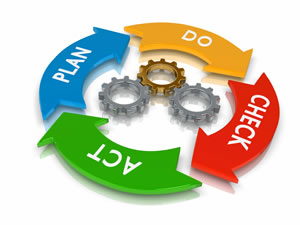
\includegraphics[scale=1.8]{./content/Immagini/PDCA}
		\caption{Il ciclo PDCA}
	\end{figure}
\end{itemize}